\section{Processi di supporto}
	\subsection{Documentazione}
		\subsubsection{Scopo}
			Lo scopo di questa sezione è definire gli standard e le regole che riguardano la stesura e l'approvazione dei documenti.
			I documenti sono consultabili nelle apposite sezioni della \glock{repository}:\\
			\\
			\centerline{\url{https://github.com/DPCMGroup/dpcm2077-docs}}
		\subsubsection{Aspettative}
			Si vuole fornire uno strumento unico per tutto il gruppo per ogni fase del ciclo di vita dei documenti, in modo da avere una documentazione uniforme e aderente agli standard e regole sotto riportate.
		\subsubsection{Descrizione}
			Questa sezione fornisce i dettagli su come deve essere redatta, verificata, e approvata la documentazione. Tutte le norme descritte devono essere rispettate in pieno in tutti i documenti, sia interni che esterni, rilasciati durante il ciclo di vita del software.
		\subsubsection{Attività}
			\paragraph{Implementazione del processo}
				\subparagraph{Ciclo di vita}
					Ogni documento viene creato basandosi sul seguente ciclo di vita:
					\begin{itemize}
					\item \textbf{stesura:} il documento viene creato da uno o più redattori seguendo le regole presenti in questo documento. Una volta terminata la stesura i redattori autorizzeranno l'avanzamento del documento all'attività successiva.
					\item \textbf{verifica:} viene effettutato da uno o più verificatori un controllo sul documento sia per quanto riguarda la stesura corretta, sia per un controllo semantico e sintattico seguendo le norme di progetto. Terminato il controllo se il documento dovesse essere corretto, i verificatori autorizzeranno il passaggio del documento alla fase successiva, in caso contrario tornerà alla prima fase, con le indicazioni delle parti da emendare.
					\item \textbf{approvazione:} è l'ultima fase del ciclo di vita del documento. In questa fase il responsabile autorizza o meno il rilascio il documento.
					\end{itemize}
				Il responsabile ha facoltà di intervenire, in ogni momento del ciclo di vita del documento, dando indicazioni se interpellato o per sua volontà.
				\subparagraph{Documenti ufficiali}
					Si dicono ufficiali i documenti che:
					\begin{itemize}
						\item sono stati revisionati, verificati e approvati;
						\item sono gli unici rilasciabili all'esterno del gruppo di progetto.
					\end{itemize}
					
					I documenti ufficiali che saranno prodotti sono:
					\begin{description}
						\item[\textbf{Studio di fattibilità:}] ha l'obiettivo di descrivere in modo breve ogni capitolato, mostrando quelli che per \textit{DPCM 2077} possono essere punti di forza, aspetti interessanti o criticità. I destinatari di questo documento sono i membri del gruppo \textit{DPCM 2077}.
						\item[\textbf{Piano di progetto:}] stabilisce e documenta tutti gli aspetti del nostro progetto organizzandoli in modo da raggiungere i risultati nel modo più efficace ed efficiente possibile. Organizza le attività, ne analizza i rischi, e le associa ai membri del gruppo. I destinatari di questo documento sono il committente e il proponente oltre al gruppo \textit{DPCM 2077}. 
						\item[\textbf{Piano di qualifica:}] espone e descrive i criteri di valutazione della qualità adottati dal gruppo. I destinatari di questo documento sono il committente e il proponente oltre al gruppo \textit{DPCM 2077}. 
						\item[\textbf{Analisi dei requisiti:}] ha lo scopo di definire le funzionalità che il nostro progetto deve offrire e quindi i requisiti che devono essere soddisfatti. I destinatari di questo documento sono il committente e il proponente oltre al gruppo \textit{DPCM 2077}.
						\item[\textbf{Verbali:}] hanno lo scopo di riassumere in modo conciso i contenuti delle riunioni e soprattutto le decisioni prese da \textit{DPCM 2077}.
						\item[\textbf{Glossario:}] il documento è composto da un elenco ordinato di tutti i termini usati nella documentazione che il gruppo ritiene necessitino di una definizione esplicita, al fine di rimuovere ogni ambiguità. I destinatari di questo documento sono il committente e il proponente oltre al gruppo \textit{DPCM 2077}.
					\end{description}
					
			\paragraph{Sviluppo e design}
				\subparagraph{Template LaTeX}
					Il gruppo ha deciso di utilizzare un template LaTeX per la stesura di tutti i documenti in modo da garantire uniformità tra questi.	
				\subparagraph{Struttura generale dei documenti}		
					Un file "main.tex" provvederà a raccogliere tutte le sezioni, pacchetti e comandi necessari per la sua compilazione. Tutti i documenti hanno una struttura predefinita e determinata.
				\subparagraph{Frontespizio}	
					Il frontespizio conterrà il logo e il nome del gruppo, il nome del documento, il nome del progetto al quale si riferisce e tutte le informazioni riguardanti il documento in sè quali:
					\begin{itemize}
						\item \textbf{versione:} versione attuale del documento;
						\item \textbf{uso:} destinazione d'uso del documento, che potrà essere "interno" o "esterno";
						\item \textbf{stato:} attuale stato del documento, che potrà essere "in redazione" o "approvato";
						\item \textbf{destinatari:} destinatari del documento;
						\item \textbf{redazione:} lista dei membri del gruppo che si sono occupati della stesura dello specifico documento;
						\item \textbf{verifica:} lista dei membri del gruppo che si sono occupati della verifica dello specifico documento;
						\item \textbf{approvazione:} nominativo del membro del gruppo che ha approvato il documento per il rilascio.
					\end{itemize}
					
				\subparagraph{Registro modifiche}
					Il registro delle modifiche consiste in una tabella contenente le informazioni riguardanti il ciclo di vita del documento. Più precisamente, la tabella riporta per ogni modifica:
					\begin{itemize}
						\item \textbf{versione:} versione del documento relativa alla modifica effettuata;
						\item \textbf{descrizione:} breve descrizione della modifica effettuata;
						\item \textbf{data:} data in cui la modifica è stata effettuata;
						\item \textbf{autore:} nominativo della persona che ha effettuato la modifica;
						\item \textbf{ruolo:} ruolo della persona che ha effettuato la modifica.
					\end{itemize}
				\subparagraph{Indice}
				L’indice delle sezioni fornisce al fruitore una visione complessiva della struttura del documento, permette di orientarsi tra i contenuti e di individuare la posizione delle varie parti. Ogni documento presenta un indice dei contenuti, subito dopo il registro delle modifiche.
				\subparagraph{Verbali}
				I verbali sono suddivisi nelle seguenti sezioni:
				\begin{itemize}
						\item \textbf{introduzione:} essa contiene:
							\begin{itemize}
								\item \textbf{luogo:} la piattaforma online in cui si svolge l'incontro;
								\item \textbf{data:} data dell'incontro;
								\item \textbf{ora di inizio:} l'ora dell'inizio dell'incontro in formato HH:MM;
								\item \textbf{ora di fine:} l'ora della fine dell'incontro in formato HH:MM;
								\item \textbf{ordine del giorno:} consiste in una lista degli argomenti che il gruppo si è proposto di discutere durante l'incontro;
								\item \textbf{presenze:} contiene la lista dei presenti e la lista degli assenti con eventuale giustifica;
							\end{itemize}
							\item \textbf{svolgimento:} per ogni punto presente nell'ordine del giorno, viene riportato un riassunto di ciò che è stato trattato durante l'incontro;
							\item \textbf{tracciamento delle decisioni:} è un riepilogo in formato tabellare delle decisioni prese durante l'incontro; esso è composto da:
							\begin{itemize}
								\item \textbf{codice:} del tipo ``AAAA-MM-GG\_ X.Y" dove la prima parte indica la data dell'incontro a cui fa riferimento seguita da un numero che indica il numero del verbale(X) ed un secondo numero che indica il punto all'ordine del giorno a cui si riferisce(Y);
								\item{ \textbf{descrizione:} breve descrizione riassuntiva della decisione presa riguardante il punto dell'ordine del giorno.}
								\end{itemize}
					\end{itemize}
				\subparagraph{Glossario}
				Il \textit{Glossario} segue la struttura principale di tutti gli altri documenti. Il contenuto è composto da una lista, che segue l'ordine lessicografico, di termini seguiti dalla loro spiegazione. I termini che si trovano nel glossario sono presenti all'interno di almeno uno dei documenti e ne viene data la spiegazione in quanto trattano argomenti ambigui e/o di poca comprensione, oppure hanno natura specifica o sono acronimi. 
				\subparagraph{Lettere}
				La \textit{Lettera di presentazione} dovrà seguire il classico layout per lettere, il che implica la presenza dei mittenti e destinatari, il logo del gruppo e la lista di tutti i documenti rilasciati, nonché il preventivo per il progetto.
			\paragraph{Norme tipografiche}
				\subparagraph{Formati comuni}
					\begin{itemize}
						\item \textbf{data:} viene utilizzato lo standard ISO 8601, esempio 2020-01-22, per la rappresentazione di tutte le date presenti della documentazione;
						\item \textbf{ora:} viene utilizzato il formato HH:MM;
					\end{itemize}
				\subparagraph{Grammatica e sintassi}
					\begin{itemize}
						\item prediligere frasi brevi, con basso livello di subordinazione e intorno a un singolo argomento;
						\item attenzione alla concordanza fra tempi verbali: il tempo verbale deve essere coerente non solo nel singolo documento / capitolo che si scrive ma globalmente. Es. tendenzialmente non si utilizza il presente in un 								verbale e dopo due righe il passato prossimo ma solo il passato prossimo (si registrano decisioni prese) né tantomeno si cambia il tempo verbale fra capitoli appartenenti allo stesso documento;
						\item l'uso della 'd' eufonica dovrebbe essere limitato ai casi di incontro della stessa vocale (es. ed ecco, ad andare, ad ascoltare, etc...). Per esempio non va bene ed organizzazione;
						\item attenzione agli accenti: perché 	e non perchè oppure perche';
						\item tutti i segni d’interpunzione seguono immediatamente la parola precedente e vanno separati con uno spazio da quella successiva;
						\item In genere le parentesi racchiudono un inciso nel discorso (cioè una parte che si può omettere, come questa). Inoltre, attenzione agli spazi: “esempio (x, y, z) esempio” e non esempio(x,  y,z)esempio;
						\item acronimo tutto maiuscolo. Se si usa acronimo prima volta va specificato in esteso;
						\item nomi con l'iniziale maiuscola;
						\item Per gli elenchi puntati:
							\begin{itemize}
								\item ogni voce di un elenco semplice (i cui elementi sono costituiti da un solo enunciato) comincia con l’iniziale minuscola e termina con il punto e virgola tranne l’ultima, seguita dal punto fermo;
								\item ogni voce di un elenco complesso (in cui almeno uno degli elementi sia composto da più di un enunciato) comincia con l’iniziale maiuscola (anche dopo il segno di due punti) e termina con il punto 										fermo;
								\item l’iniziale maiuscola è permessa se si fa riferimento a nomi di documentazione, nomi propri di persona, etc.;
								\item non bisogna per forza uniformare tutti gli elenchi di un documento a criteri stabiliti a priori: l’importante è essere coerenti volta per volta.
							\end{itemize}
						\item \textbf{grassetto}: per evidenziare parole importanti.
					\end{itemize}
				\subparagraph{Lettere maiuscole}
				Tutti i titoli vanno con iniziale maiuscola. Usare le maiuscole solo in caso di nomi propri e documenti (es Analisi dei requisiti. non analisi dei requisiti o Analisi dei Requisiti. È consentita l'uso della sigla AdR).
				\subparagraph{Sigle}
				Il progetto prevede la redazione di un insieme di documenti, suddivisi in documenti interni e documenti esterni. Essi sono elencati di seguito con le rispettive sigle.\\
				I documenti esterni sono:
				\begin{itemize}
				\item \textbf{Analisi dei requisiti - AdR};
				\item \textbf{Piano di Progetto - PdP};
				\item \textbf{Piano di Qualifica - PdQ};
				\item \textbf{Manuale Utente - MU};
				\item \textbf{Manuale Sviluppatore - MS}.
				\end{itemize}
				I documenti interni sono:
				\begin{itemize}
				\item \textbf{Glossario: G};
				\item \textbf{Norme di Progetto: NdP};
				\item \textbf{Studio di Fattibilità - StF}.
				\end{itemize}
				Per quanto riguarda il \textbf{Verbale - V} questo può essere sia interno sia esterno.
\\
				Le diverse fasi del progetto sono: 
				\begin{itemize}
				\item \textbf{Revisione dei Requisiti - RR}: studio iniziale del C1;
				\item \textbf{Revisione di Progettazione - RP}: riguarda la definizione dell'architettura del software e della sua fattibilità;
				\item \textbf{Revisione di Qualifica - RQ}: riguarda la definizione dettagliata e la codifica del prodotto;
				\item \textbf{Revisione di Accettazione - RA}: se il prodotto soddisfa i requisiti del proponente, viene accettato e rilasciato.
				\end{itemize}
	\subsubsection{Strumenti}
			\paragraph{LaTeX}
			Lo strumento scelto per la scrittura di documenti è \LaTeX{}, un linguaggio che permette di scrivere documenti in modo ordinato, modulare e collaborativo.
			\paragraph{Google Drive}
			Si utilizza \glock{Google Drive} per salvare file utili al gruppo di qualunque genere.
			\paragraph{Diagrammi}
				I software utilizzati per la realizzazione dei diagrammi sono i seguenti:
				\begin{itemize}
					\item \textbf{StarUML:} per la realizzazione di \glock{diagrammi UML};
					\item \textbf{GanttProject:} applicazione open source per la realizzazione di \glock{diagrammi di Gantt} che mostrano lo svolgimento delle attività.
				\end{itemize}
			
	\subsection{Gestione della Configurazione}
		\subsubsection{Scopo}
			La gestione della configurazione definisce i principi normativi utili a predisporre il \glock{workspace} per tutto il gruppo, semplificando e automatizzando la conservazione dei documenti e delle componenti software, che andranno a formare il prodotto finale.
		\subsubsection{Versionamento}
			\paragraph{Codice di versione del documento}
			Ogni documento deve avere una storia, ricostruibile tramite le sue versioni. Ogni numero di versione è così composto:\\
			\centerline{\textbf{X.Y.Z}}
			\begin{itemize}
			\item \textbf{X}: rappresenta una versione stabile del documento, resa tale dopo l'approvazione dal responsabile di progetto:
				\begin{itemize}
		   			\item inizia da 0;
		   			\item viene incrementato dal responsabile di progetto all'approvazione del documento.
		  		\end{itemize}
		  	\item \textbf{Y}: rappresenta una versione parzialmente stabile del documento che è stata approvata parzialmente dal responsabile di progetto:
		  		\begin{itemize}
		   			\item inizia da 0;
		   			\item viene incrementato dal responsabile a ogni approvazione parziale. Per approvazione parziale si intende che una o più sezioni del documento sono pronte per il rilascio all'esterno del gruppo, e che quindi non è 								necessario attendere l'approvazione totale del documento da parte del responsabile per poterle rilasciare.
		   			\item quando viene incrementato X, viene riportato a 0.
		   		\end{itemize}
		   	\item \textbf{Z}: rappresenta una versione instabile del documento in fase di lavorazione da parte dei redattori:
		   		\begin{itemize}
		   			\item inizia da 0;
		   			\item viene incrementato dal redattore a ogni modifica; 
		   			\item quando viene incrementato X, viene riportato a 0.
		   		\end{itemize}
			\end{itemize}
			
			\paragraph{Versionamento con GitHub}
	Il repository fa uso di un Version Control System (VCS) di tipo distribuito sotto il motore \textit{Git}, che permette la condivisione dal locale al remoto del proprio spazio di lavoro su un luogo comune.\\
		Attraverso l'utilizzo di un web browser, è possibile collegarsi a \textit{GitHub} e controllare i file contenuti in un repository. 
			\paragraph{Repository}
			Ci sono due tipi di repository la cui struttura è identica e raccolgono i file sorgenti per la compilazione dei documenti, suddivisi tra esterni e interni:
			\begin{itemize}
		   			\item \textbf{locale}: ogni membro del gruppo lavora sui file clonati dal repository remoto nel proprio computer;
		   			\item \textbf{remoto}: pubblicato su \textit{GitHub}, contiene il lavoro svolto da ogni componente e che viene condiviso con i membri di DPCM 2077.
		   	\end{itemize}
		   	\paragraph{Configurazione del workflow}
	Si è deciso di stabilire il seguente canone di \glock{workflow} per quanto concerne la documentazione:
	\begin{itemize}
	\item \textbf{master branch:} branch principale su cui vengono fatti i rilasci ad ogni \glock{milestone};
	\item \textbf{develop branch:} branch di sviluppo su cui viene fatta integrazione di nuove funzionalità concluse;
	\item \textbf{feature/... branch:} i puntini saranno sostituiti dal nome del documento a cui si riferisce il branch. Questo tipo di branch viene aperto al momento della crezione del documento a cui si riferisce e chiuso solo al momento dell'approvazione e rilascio.
	\end{itemize}
		   	
	\subsection{Garanzia della Qualità}
		\subsubsection{Scopo}
		Lo scopo è di garantire che il prodotto e i servizi offerti rispettino gli obiettivi di qualità e che i bisogni del proponente siano soddisfatti.
		\subsubsection{Aspettative}
		Attraverso la gestione della qualità si intende ottenere:
		\begin{itemize}
			\item un prodotto software di qualità;
			\item una documentazione completa e facilmente comprensibile per tutti;
			\item dei processi che seguano dei punti ben specificati per l'analisi di qualità;
			\item una comunicazione chiara e semplice delle problematiche relative alla qualità tra i membri del team;
			\item una registrazione dei risultati ottenuti.
		\end{itemize}
		\subsubsection{Descrizione}
		Per una presentazione dettagliata della gestione della qualità si fa riferimento al Piano di Qualifica v.2.?.?, dove vengono presentati:
		\begin{itemize}
			\item gli standard utilizzati;
			\item i processi di interesse negli standard;
		\end{itemize}
		\subsubsection{Controllo qualità di prodotto}
		La qualità di prodotto viene garantita dai processi di verifica e validazione e dal rispetto delle norme.
		\begin{itemize}
			\item \textbf{Verifica}: accerta che l’esecuzione delle attività di processo siano corrette;
			\item \textbf{Validazione}: accerta che il prodotto rispecchi le aspettative, utilizzando un metodo sistematico, disciplinato e quantificabile;
			\item \textbf{Norme}:   il  prodotto  deve  rispettare  le  norme  e  gli  strumenti  descritti  all’interno  di  questo documento.
		\end{itemize}
		Per ogni prodotto vengono descritti: 
		\begin{itemize}
			\item le metriche da utilizzare;
			\item gli obiettivi da perseguire.
			\end{itemize}
		\subsubsection{Controllo qualità di processo}
		La qualità di processo viene migliorata per tutto il ciclo di vita del software attraverso i principi di efficacia ed efficienza mirati al prodotto.
			Nello specifico definiamo quanto segue:
			\begin{itemize}
				\item \textbf{Efficacia:} si richiede un prodotto che soddisfi le richieste del proponente;
				\item \textbf{Efficienza:} i processi devono convergere con costi ridotti in termini di risorse a pari qualità di prodotto.
			\end{itemize}
			Per ogni processo vengono descritti: 
			\begin{itemize}
			\item le metriche da utilizzare;
			\item gli intervalli entro i quali le misurazioni sono ritenute preferibili e accettabili.
			\end{itemize}
		\subsubsection{Attività}
		Le tre attività principali sono:
		\begin{itemize}
		\item \textbf{Pianificazione}: porsi degli obiettivi, definire le strategie per raggiungerli e predisporre persone e risorse per raggiungere gli obiettivi nel modo più efficiente possibile;
		\item \textbf{Valutazione}: applicare i criteri misurando e monitorando i risultati;
		\item \textbf{Reazione}: sulla base dei risultati applicare le proprie strategie, criteri e piani.
		\end{itemize}
		\subsubsection{Strumenti}
		Gli strumenti che garantiscono la qualità sono identificati negli standard \textbf{ISO-12207} e \textbf{ISO-9126}.
	\subsection{Verifica}
		\subsubsection{Scopo}
			Il processo di verifica ha come scopo la realizzazione di un prodotto corretto, basandosi sulle richieste del committente/proponente e sulle norme definite in questo documento.
		\subsubsection{Aspettative}
		Lo svolgimento del processo di verifica sarà garantito seguendo determinati punti:
    \begin{itemize}
        \item definizione di criteri di accettazione;
	\item prescrizione delle attività di verifica con relativa documentazione;
	\item test di verifica;
	\item correzione di eventuali \glock{difetti}.
	\item dopo la verifica il prodotto è in uno stato stabile;
	\item rende possibile la validazione.
    \end{itemize}
    	\subsubsection{Descrizione}
		Il processo di verifica prende in input ciò che è già stato prodotto e lo restituisce in uno stato conforme alle aspettative. Per ottenere tale risultato vengono effettuati processi di analisi e test.
		\subsubsection{Attività}
			\paragraph{Analisi}
			Il processo di analisi si suddivide in:
			\begin{itemize}
			\item \textbf{Statica}: effettuata su documenti e codice, ha lo scopo di valutarne la conformità alle regole qui descritte, la mancanza di errori sintattici e grammaticali e la coesione dei componenti. Alcuni controlli sono da fare ad esempio sulle date, sulla forma dei verbi, sulla punteggiatura. Verranno usati due tipi di analisi statica:
			\begin{itemize}
				\item \textbf{\glock{Walkthrough}}: i vari componenti di DPCM 2077 analizzano gli oggetti nella loro totalità per cercare anomalie, senza sapere inizialmente se vi siano difetti;
				\item \textbf{\glock{Inspection}}: i verificatori usano le liste di controllo per fare ispezione cercando errori specifici in parti specifiche.
			\end{itemize}
			\begin{figure}[H]
	\centering
	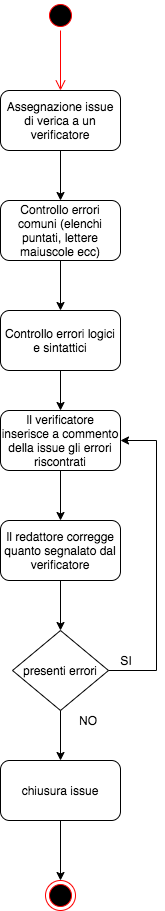
\includegraphics[width=2.5cm]{res/images/verifica.png}
	\caption{Verifica di un documento}
	\label{fig:Verifica di un documento}
\end{figure}
			\item \textbf{Dinamica}: tecnica di analisi del prodotto software che richiede la sua esecuzione. Viene effettuata mediante dei test che verificano se il prodotto funziona o se ci sono anomalie.
			\end{itemize}
			\paragraph{Test}
			I test rappresentano l'attività fondamentale dell'analisi dinamica. Lo scopo dei test è dimostrare che il codice scritto funzioni correttamente e che non presenti errori. 
			Per ogni test devono essere definiti i seguenti parametri: 
			\begin{itemize}
			\item \textbf{ambiente:} sistema hardware e software sul quale verrà eseguito il test;
			\item \textbf{stato iniziale:} stato iniziale dal quale il test viene eseguito;
			\item \textbf{input:} dati in ingresso immessi;
			\item \textbf{output:} dati in uscita attesi;
			\item \textbf{istruzioni aggiuntive:} ulteriori istruzioni su come deve essere eseguito il test e su come interpretare i risultati ottenuti.
			\end{itemize}
			Dei test ben scritti, per definirsi tali, devono:
			\begin{itemize}
			\item essere ripetibili;
			\item specificare l'ambiente di esecuzione;
			\item identificare input e output richiesti;
			\item controllare la presenza di effetti indesiderati;
			\item fornire informazioni sui risultati dell’esecuzione sotto forma di file di log.
			\end{itemize}
			Per elencare le specifiche dei test si è scelta una rappresentazione tabellare contenente il codice del componente da testare, la descrizione dei test, il suo stato di avanzamento e il risultato del test.
			Di seguito la nomenclatura dello stato del test:
			\begin{itemize}
				\item \textbf{I}: il test è stato implementato;
				\item \textbf{NI}: il test non è stato implementato.
			\end{itemize}			
			Di seguito la nomenclatura del risultato del test:
			\begin{itemize}
				\item \textbf{S}: il test si è concluso con successo;
				\item \textbf{F}: il test ha fallito.
			\end{itemize}		
			Di seguito sono spiegati i diversi test del software.
			\subparagraph{Test di unità}
			I test di unità si eseguono su unità di software. Questi test si concentrano sul funzionamento delle unità individuali. Dati gli input possibili in un'unità, si suddividono gli input in partizioni di equivalenza e si prova se gli input attesi danno gli output previsti.
			Questa tipologia di test verrà classificata nel seguente modo:
			\begin{center}
				\textbf{TU[Identificativo]}
			\end{center}
			dove:
			\begin{itemize}
				\item \textbf{Identificativo}: numero progressivo univoco incrementale, inizia da 1.
			\end{itemize}
			\subparagraph{Test di integrazione}
			I test d’integrazione verificano la correttezza delle interfacce. Rappresentano l’estensione logica dei test d’unità e sono i predecessori dei test di sistema. Vengono svolti aggregando due o più unità già testate in un unico componente ed espandendo, di fatto, i test di moduli di un gruppo con quelli di altri gruppi. Ogni test prevede vi siano almeno un paio di componenti correlate per sottoporre a verifica tutte le unità che compongono un processo.
			Questa tipologia di test verrà classificata nel seguente modo:
			\begin{center}
				\textbf{TI[Identificativo]}
			\end{center}
			dove:
			\begin{itemize}
				\item \textbf{Identificativo}: numero progressivo univoco incrementale, inizia da 1.
			\end{itemize}
			\subparagraph{Test di sistema}
			Una volta integrati tutti i suoi componenti il sistema viene testato nella sua interezza. Ci si concentra sulle interazioni tra le parti, sul comportamento delle caratteristiche del sistema e sulla copertura di tutte le funzionalità. In questa fase ci si assicura che il sistema rispetti tutte le specifiche definite nell'\textit{Analisi dei Requisiti}.
			Questa tipologia di test verrà classificata nel seguente modo:
			\begin{center}
				\textbf{TS[Priorità][Tipologia][Identificativo]}
			\end{center}
			dove:
			\begin{itemize}
				\item \textbf{Priorità}: indica la priorità del requisito associato al test:
				\begin{itemize}
					\item \textbf{\textit{1}}: obbligatorio, ossia irrinunciabile;
					\item \textbf{\textit{2}}: desiderabile, non strettamente necessario;
					\item \textbf{\textit{3}}: opzionale, ossia relativamente utile o contrattabile in corso d'opera.
				\end{itemize}
				\item \textbf{Tipologia} : indica la tipologia del requisito associato al test:
				\begin{itemize}
					\item \textbf{\textit{F}}: funzionale;
					\item \textbf{\textit{P}}: prestazionale;
					\item \textbf{\textit{Q}}: qualitativo;
					\item \textbf{\textit{V}}: vincolo.
				\end{itemize}
				\item \textbf{Identificativo}: numero progressivo univoco incrementale, inizia da 1.
			\end{itemize}
			\subparagraph{Test di regressione}
			Si effettua a seguito di una modifica del sistema e consiste nella riesecuzione dei test esistenti.
			\subparagraph{Test di accettazione}
			Anche detto "test di collaudo", è simile al test di sistema per l’oggetto testato, ma viene eseguito con la partecipazione dei committenti. Verifica il prodotto e, in particolare, il soddisfacimento del cliente. Il superamento del test di collaudo garantisce che il software è pronto per essere rilasciato.
			Questa tipologia di test verrà classificata nel seguente modo:
			\begin{center}
				\textbf{TA[Priorità][Tipologia][Identificativo]}
			\end{center}
			dove:
			\begin{itemize}
				\item \textbf{Priorità}: indica la priorità del requisito associato al test:
				\begin{itemize}
					\item \textbf{\textit{1}}: obbligatorio, ossia irrinunciabile;
					\item \textbf{\textit{2}}: desiderabile, non strettamente necessario;
					\item \textbf{\textit{3}}: opzionale, ossia relativamente utile o contrattabile in corso d'opera.
				\end{itemize}
				\item \textbf{Tipologia} : indica la tipologia del requisito associato al test:
				\begin{itemize}
					\item \textbf{\textit{F}}: funzionale;
					\item \textbf{\textit{P}}: prestazionale;
					\item \textbf{\textit{Q}}: qualitativo;
					\item \textbf{\textit{V}}: vincolo.
					\item \textbf{Identificativo}: numero progressivo univoco incrementale, inizia da 1.
				\end{itemize}
			\end{itemize}
			\subsubsection{Strumenti}
			\paragraph{Verifica ortografica}
			Per la verifica ortografica dei documenti scritti in \LaTeX{} si utilizzerà lo strumento di correzione automatica presente negli editor Texmaker e TexStudio.

	\subsection{Validazione}
		\subsubsection{Scopo}
			Lo scopo del processo di validazione consiste nel garantire che il prodotto soddisfi il compito per cui è stato creato e che quindi rispecchi le richieste del committente.
		\subsubsection{Aspettative}
			La corretta esecuzione di tale processo consente di individuare:
			\begin{itemize}
				\item una procedura di validazione;
				\item i criteri per la validazione;
				\item la conformità del prodotto finito.
			\end{itemize}
		\subsubsection{Descrizione}
			Il processo di validazione consiste nell’identificare gli oggetti da validare e valutare che i risultati rispettino le aspettative.
		\subsubsection{Attività}
		   	Le attività di validazione sono:
		   	\begin{enumerate}
		   		\item eseguire i test sul prodotto;
		   		\item i verificatori eseguono i test e stendono un resoconto sui risultati;
		   		\item se i risultati non sono soddisfacenti si ritorna al primo punto e si rieseguono i test;
		   		\item i risultati vengono inviati al proponente.
		   	\end{enumerate}
			
